
\begin{enumerate}[label=\arabic*.,ref=\theenumi]
    \item In \figref{fig:fig1.png} if tangents $\vec{PA}$ and $\vec{PB}$ from an external point $P$ to a circle with centre $O$ , are inclined to each other at an angle of $80^{\degree}$, then $\angle AOB$ is equal to
 \begin{figure}[H]
        \centering
        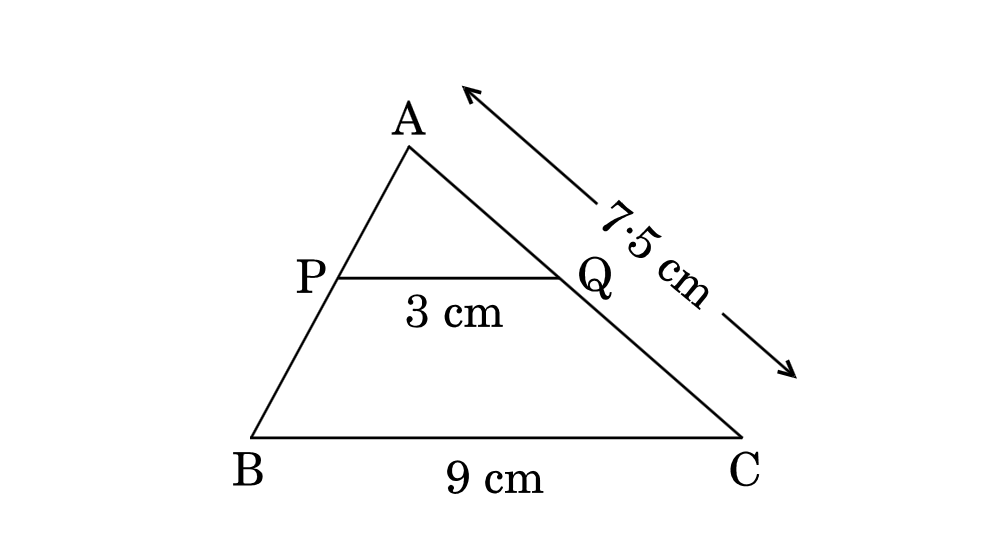
\includegraphics[width = \columnwidth]{figs/figure1.png}
        \caption{Tangents $PA$ and $PB$}
        \label{fig:fig1.png}
    \end{figure}
    \begin{enumerate}
        \item $100^{\degree}$
        \item $60^{\degree}$
        \item $100^{\degree}$
        \item $100^{\degree}$
    \end{enumerate}

    \item  Two concentric circles are of radii $4 cm$ and $3 cm$. Find the length of the chord of the larger circle which touches the smaller circle.

    \item  In \figref{fig:fig2.png}, a triangle $ABC$ with $\angle AOB$ is shown. Taking $AB$ as diameter, a circle has been drawn intersecting $AC$ at point $P$. Prove that the tangent drawn at point $P$ bisects $BC$. 
	        \begin{figure}[H]
 %       \centering
        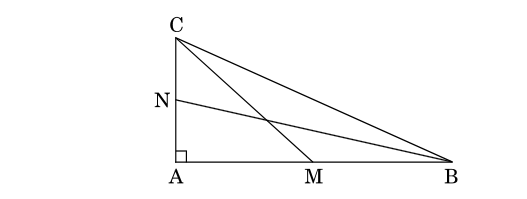
\includegraphics[width = \columnwidth]{figs/figure2.png}
        \caption{Concentric circles}
        \label{fig:fig2.png}
               \end{figure}
    \item  Prove that a Parallelogram circumscribing a circle is a rhombus.
     \item  In \figref{fig:fig3.png}, two circles with centres at $O$ and $O$ of radii $2r$ and $r$ respectively, touch each other internally at $A$. A chord $AB$ of the bigger circle meets the smaller circle at $C$. Show that  $C$ bisects $AB$.
    \begin{figure}[H]
        \centering
        \includegraphics[width = \columnwidth]{figs/figure3.png}
        \caption{Two circles with center}
        \label{fig:fig3.png}
    \end{figure}  
    
    \item In \figref{fig:fig4.png}, $O$ is centre of a circle of radius $5 cm$. $PA$ and $BC$ are tangents to the circle at $A$ and $B$ respectively. If $OP = 13 cm$, then find the length of tangents $PA$ and $BC$.
     \begin{figure}[H]
        \centering
        \includegraphics[width = \columnwidth]{figs/figure4.png}
        \caption{The center of the circle of radius 5 cm}
	     \label{fig:fig4.png}
    \end{figure}
    
    \item In two concentric circles, a chord of length $48 cm$ of the larger
circle is a tangent to the smaller circle, whose radius is $7 cm$. Find the radius of the larger circle. 
    \item At a point on the level ground, the angle of elevation of the top
of a vertical tower is found to be $\alpha$, such that $\tan \alpha =\frac{5}{12} $. On walking $192 m$ towards the tower, the angle of elevation $\beta$ is such that $\tan \beta=\frac{3}{4}$. Find the height of the tower. 
    \end{enumerate}
\end{document}
